% === Dokumentklasse ==========================================================
\documentclass[%
    a4paper,							% A4
    12pt,								% Schriftgröße 12
    twoside,							% zweiseitig
    fleqn								% Formeln linksbündig ausrichten
]{book}


% === Grundlegende Pakete =====================================================
\usepackage{etoolbox}					% portiert viele nützliche Sachen aus e-TeX (z.B. booleans, ifs)
\usepackage[							% erweiterte Angabe von Farben
    pdftex,								% Farbtreiber auswählen
    dvipsnames							% vordefinierte Farben laden
]{xcolor}								% erweiterte Angabe von Farben
\usepackage{xparse}						% high-level Interface für Dokumentbefehle wie \NewDocument(Command,Environment)

\usepackage[utf8]{inputenc}				% Kodierung der *.tex Dateien ist UTF-8 nicht ISO-8859-1
\usepackage{cmap}						% character map tables -> pdf Inhalt wird besser durchsuch- und kopierbar
\usepackage[T1]{fontenc}				% OT1 encoding für deutsche Sonderzeichen -> pdf Inhalt kann Sonderzeichen durchsucht werden
\usepackage{lmodern}					% Latin-Modern-Schriftart (Computer Modern in Verbindung mit OT1 führt zu Bitmap-Fonts auf Windows)
\usepackage{microtype}					% mikrotypografische Einstellungen, die den gesetzten Text nochmals wesentlich verbessern (weniger badboxes)


% === Benutzerdefinierte Einstellungen ========================================
% === Art der Arbeit ==========================================================
% von den nachfolgenden Blöcken bitte den richtigen auswählen und die anderen auskommentieren/löschen

% --- Diplom ----------
%\newcommand{\settingsDegree}{{Diplom}}
%\newcommand{\settingsDegreeName}{{Diplominformatiker}}
%\newcommand{\settingsDegreeName}{{Diplomingenieur}}

% --- Bachelor ----------
% \newcommand{\settingsDegree}{{Bachelor}}
% \newcommand{\settingsDegreeName}{{Bachelor of Science}}

% --- Master ----------
\newcommand{\settingsDegree}{{Master}}
\newcommand{\settingsDegreeName}{{Master of Science}}

% === Name, Abgabedatum und Sprache der Arbeit ================================
\newcommand{\settingsName}{{Pierre Helbing}}
\newcommand{\settingsFinishDate}{{DD.MM.YYYY}}
\newcommand{\settingsLanguage}{german}   		% german / american

% === Weitere Einstellungen ===================================================
% --- Suchpfad (Unterverzeichnis) für eingebundene Grafiken ----------
\newcommand{\settingsGraphicsPath}{image/}

% --- Hinweiskapitel ----------
\newbool{settingsWithHints}
\setbool{settingsWithHints}{false}				% true / false

% --- Zeilennummern ----------
\newbool{settingsWithLineNumbers}
\setbool{settingsWithLineNumbers}{false}			% true / false

% --- Todos ----------
\newbool{settingsWithTodos}
\setbool{settingsWithTodos}{true}				% true / false

% --- Anzahl an Nummerierungsebenen im Text und Inhaltsverzeichnis ----------
% 1: \section
% 2: \section + \subsection
% Achtung: 3 oder 4 nur nach Absprache mit Betreuer !
% 3: \section + \subsection + \subsubsection
% 4: \section + \subsection + \subsubsection + \paragraph
\setcounter{secnumdepth}{2}
\setcounter{tocdepth}{2}

% --- Anforderungen ----------

\usepackage{tabularx}
\usepackage{multicol}
\newenvironment{myreq}[1]{%
    \setlist[description]{font=\normalfont\color{darkgray}}%
    \begin{tcolorbox}[colframe=black,colback=white, sharp corners, boxrule=1pt]%
        \bfseries\color{blue}%
        \begin{description}#1}%
            {\end{description}\end{tcolorbox}}

\newcommand{\threeinline}[3]{\begin{multicols}{3}#1 #2 #3\end{multicols}}
\newcommand{\twoinline}[2]{\begin{multicols}{2}#1 #2\end{multicols}}

\newcommand{\reqno}{\item[Requirement \#:]}
\newcommand{\reqtype}{\item[Requirement Type:]}
\newcommand{\reqevent}{\item[Event/BUC/PUC \#:]}
\newcommand{\reqdesc}{\item[Description:]}
\newcommand{\reqrat}{\item[Rationale:]}
\newcommand{\reqorig}{\item[Originator:]}
\newcommand{\reqfit}{\item[Fit Criterion:]}
\newcommand{\reqsatis}{\item[Customer Satisfaction:]}
\newcommand{\reqdissat}{\item[Customer Dissatisfaction:]}
\newcommand{\reqdep}{\item[Dependencies:]}
\newcommand{\reqconf}{\item[Conflicts:]}
\newcommand{\reqmater}{\item[Materials:]}
\newcommand{\reqhist}{\item[History:]}
\usepackage{multicol}
\usepackage{multirow}
\usepackage[dvipsnames]{xcolor}
\usepackage{enumitem}
\usepackage{tcolorbox}

% === Übersetzungen ===========================================================
% Definitionen je nach \mylanguage (siehe NIKR_settings.tex)
\ifdefstring{\settingsLanguage}{german}{%
    \newcommand{\acroname}{Abkürzungsverzeichnis}	% Name für Abkürzungsverzeichnis
    \newcommand{\todoname}{Todo Liste}	% Name für Todo-Liste
    \newcommand{\pagename}{Seite}		% Name für Seite
}%
{%
    \newcommand{\acroname}{Acronyms}	% Name für Abkürzungsverzeichnis
    \newcommand{\todoname}{Todo list}	% Name für Todo-Liste
    \newcommand{\pagename}{page}		% Name für Seite
}%


% === Wichtige Pakete und Einstellungen =======================================
\usepackage{calc}						% ermöglicht Arithmetik in den Argumenten von Befehlen

% Einstellungen je nach \mylanguage (siehe NIKR_settings.tex)
\ifdefstring{\settingsLanguage}{german}{%
    \usepackage[ngerman]{babel}			% Spracheinstellungen (für deutsch z.B. Contents -> Inhaltsverzeichnis, etc.)
    \usepackage{bibgerm}            	% Stylefile für deutsche Literaturstellenangabe
    \bibliographystyle{gerapali}		% Stil für Literaturangaben festlegen
}%
{%
    \usepackage[american]{babel}		% Spracheinstellungen (für deutsch z.B. Contents -> Inhaltsverzeichnis, etc.)
    \bibliographystyle{apalike}			% Stil für Literaturangaben festlegen
    \frenchspacing						% einfaches Leerzeiches nach Satzende (für deutsch bereits Standard)
}%
\usepackage[%
    noadjust							% noadjust verhindert automatische Leerzeichen um die Referenz, was am Zeilenanfang zu Problemen führt
]{cite}     							% erlaubt Zeilenumbruch innerhalb von Zitierungen

\usepackage{graphicx}					% erweiterte Argumente in \in­clude­graph­ics
\graphicspath{{\settingsGraphicsPath}}	% Standard-Pfad für Bilder siehe NIKR_settings.tex

\usepackage[bf]{caption}				% erlaubt erweiterte Formatierungen in \caption (siehe unten)
\usepackage{subcaption}					% mehrere Abbildungen nebeneinander

\usepackage{amsmath}					% ermöglicht \DeclareMathOperator
\usepackage{amssymb}					% mathmatische Symbole und Sonderzeichen
\usepackage{nicefrac}					% für \nicefrac
\usepackage{nccmath}					% für \mfrac

\usepackage{icomma}						% intelligentes Komma (macht Verwendung von {,} überflüssig)
\usepackage{siunitx}					% für einheitliche Angabe von Einheiten

\usepackage{fancyhdr}					% Kopf- und Fußzeilen (siehe unten)

\usepackage{hhline}						% erweitere Rahmengestaltung in Tabellen

\usepackage[%							% Einbettung von Links im Dokument und erlaubt die Nutzugn von \url
    hyperfootnotes=false,				% keine Fußnoten als Link im Dokument (geht nicht mit footmisc)
    pagebackref=true					% Backrefs im Literaturverzeichnis
]{hyperref}           					% Einbettung von Links im Dokument und erlaubt die Nutzugn von \url
\renewcommand*{\backref}[1]{\textit{(\pagename:~#1)}}   % Format für backrefs

\usepackage[%							% erlaubt erweiterte Formatierungen von Fußnoten (siehe unten)
    multiple,							% mehrere mit Komma abtrennen
    hang								% linksbündig, \footnotemargin entscheidet über Einrückung
]{footmisc}								% erlaubt erweiterte Formatierungen von Fußnoten (siehe unten)
\patchcmd{\footref}{\ref}{\ref*}{}{}	% Hyperlink in \footref entfernen

\usepackage[nohyperlinks]{acronym}		% Abkürzungsverzeichnis

\usepackage{setspace}					% für \setstretch (ändern Zeilenabstand, aber nicht floating Umgebungen)

\usepackage[%							% Todos
    colorinlistoftodos,					% farbige Markierungen in Todo-Liste
    prependcaption,						% caption=val
    textsize=tiny,						% Schriftgröße
    linecolor=red,						% Standard-Linienfarbe für \todo
    backgroundcolor=red!25,				% Standard-Hintergrundfarbe für \todo
    bordercolor=red,					% Standard-Rahmenfarbe für \todo
    textwidth=2cm,						% Standard-Breite für \todo
]{todonotes}							% Todos
\ifbool{settingsWithTodos}{%
    \setlength{\marginparwidth}{2cm}	% sonst werden Notes am Rand nicht richtig angezeigt
    \NewDocumentCommand{\todoaddref}{O{} m}{%
        \todo[linecolor=blue,backgroundcolor=blue!25,bordercolor=blue,#1]{#2}%
    }
    \NewDocumentCommand{\todouncertain}{O{} m}{%
        \todo[linecolor=green,backgroundcolor=green!25,bordercolor=green,#1]{#2}%
    }
    \NewDocumentCommand{\todooptional}{O{} m}{%
        \todo[linecolor=cyan,backgroundcolor=cyan!25,bordercolor=cyan,#1]{#2}%
    }
    \pretocmd{\mainmatter}{\listoftodos[\todoname]{\markboth{\MakeUppercase{\todoname}}{\MakeUppercase{\todoname}}}}{}{}
}{
    \presetkeys{todonotes}{disable}{}	% disable \todo
    \NewDocumentCommand{\todoaddref}{O{} m}{}
    \NewDocumentCommand{\todouncertain}{O{} m}{}
    \NewDocumentCommand{\todooptional}{O{} m}{}
}

\usepackage[switch*,pagewise]{lineno}	% Zeilennummern
\ifbool{settingsWithLineNumbers}{%
    \renewcommand\linenumberfont{\textbf\sffamily\color{black!50}\footnotesize}
    \apptocmd{\mainmatter}{\linenumbers}{}{}
    \pretocmd{\backmatter}{\nolinenumbers}{}{}
}{}

\usepackage{placeins}					% FloatBarriers

\usepackage{enumitem}					% erweiterte Formatierung von \enumerate, \itemize und \description

\usepackage[linewidth=0.5pt]{mdframed}	% für Boxen in Hinweisen

\usepackage[ddmmyyyy]{datetime}			% Datumsangabe
\renewcommand{\dateseparator}{.}		% Punkt als Trennzeichen in Datumsangabe


% === Längen und Abstände =====================================================
% horizontales Layout
\setlength{\oddsidemargin}{0.2in}
\setlength{\evensidemargin}{0.0in}
\setlength{\textwidth}{\paperwidth - 2.2in}

% vertikales Layout
%\setlength{\topskip}{0.0cm}
\setlength{\headheight}{15.1pt}
%\setlength{\headsep}{0.0cm}
\setlength{\topmargin}{0.0cm}
\setlength{\footskip}{0.6in}
\setlength{\textheight}{\paperheight - 2.0in}
\addtolength{\textheight}{-1.0\headheight}
\addtolength{\textheight}{-1.0\headsep}
\addtolength{\textheight}{-1.0\footskip}

% Zeilenabstand
\setstretch{1.3}
\AtBeginEnvironment{tabular}{\setstretch{1.3}}

% Einrückung von Formeln
\setlength{\mathindent}{1.0cm}

% Absätze
\setlength{\parindent}{0.0cm}

% Fußnoten
\renewcommand{\footnotelayout}{\setstretch{1.2}}
\setlength\footnotemargin{10pt}

% Listen (noitemsep, nosep, ...)
\setlist{noitemsep}

\setlength{\topsep}{0.3cm}


% === Bild- und Tabellenunterschrift ==========================================
\renewcommand{\captionfont}{\small \setstretch{1.3}}
\newcommand{\NIcaption}[2]{\caption[#1]{#1\protect\\ \emph{#2}}}
\setcaptionmargin{0.75cm}


% === Abkürzungsverzeichnis ===================================================
% Verwendung vor jedem Kapitel zurücksetzen
\pretocmd{\chapter}{\acresetall}{}{}


% === Seitenstil ==============================================================
% Pagestyle plain überschreiben
\pagestyle{fancy}
% Kapitel- und Abschnittangaben ohne Punkt
\renewcommand{\sectionmark}[1]{\markright{\uppercase{\thesection~~#1}}}
\renewcommand{\chaptermark}[1]{\markboth{\uppercase{\chaptername\ \thechapter~~#1}}{}}
\fancypagestyle{plain}{%
    \fancyhead[ER]{\itshape\leftmark}%
    \fancyhead[OL]{\itshape\rightmark}%
    \fancyhead[EL,OR]{\thepage}%
    \fancyfoot[EL,OL]{}%
    \fancyfoot[EC,OC]{}%
    \renewcommand{\headrulewidth}{0.4pt}%
    \renewcommand{\footrulewidth}{0.4pt}%
}


% === Verweise ================================================================
% Klammern in Formel-Referenzen entfernen
\makeatletter
\renewcommand\tagform@[1]{\maketag@@@{\ignorespaces#1\unskip\@@italiccorr}}
\makeatother


% === Angabe von Einheiten ====================================================
\ifdefstring{\settingsLanguage}{german}{%
    \sisetup{locale=DE}		% deutsche Lokalisierung (konvertiert 1.00 automatisch zu 1,00)
}%
{%
    \sisetup{locale=US}		% englische Lokalisierung (konvertiert 1,00 automatisch zu 1.00)
}%


% === Mathematische Definitionen ==============================================
% Darstellung von Vektoren und Matrizen
\renewcommand{\vec}[1]{\underline{\mathbf{\MakeLowercase{#1}}}}		% Vektoren
\newcommand{\veci}[1]{\underline{\MakeLowercase{#1}}}				% Vektoren als Indizes
\newcommand{\mat}[1]{\underline{\mathbf{\MakeUppercase{#1}}}}		% Matrizen
\newcommand{\mati}[1]{\underline{\MakeUppercase{#1}}}				% Matrizen als Indizes
% zusätzliche mathematische Operatoren (damit sie nicht als Formelzeichen geschrieben werden)
\DeclareMathOperator{\step}{step}									% Stufenfunktion
\DeclareMathOperator{\sign}{sign}									% Vorzeichen


% === Manuelle Definition von Worttrennungen ==================================
\hyphenation{
    Convolutional
    Neural
    Net-work
    Net-works
    Ko-ef-fi-zi-ent
    Ko-ef-fi-zi-ent-en
    Drop-out
    pixel-genaue
    Patch
    Patch-größen
}


% === Pseudocode-Darstellung ==================================================
% Import nicht oben, weil \parindent zuvor gesetzt werden muss!
% siehe: https://ctan.org/pkg/algorithm2e?lang=de
\ifdefstring{\settingsLanguage}{german}{%
    \usepackage[%						% Pseudocode
        linesnumbered,					% mit Zeilennummern
        noend,							% Ende von Befehlen, wie etwa While, unterdrücken
        ruled,							% Layout
        german,							% deutsche Bezeichnung und deutsches Verzeichnis
        %onelanguage,					% Keywords übersetzen
        algochapter						% Nummerierung analog zu Abbildungen
    ]{algorithm2e}						% Pseudocode
}{%
    \usepackage[%						% Pseudocode
        linesnumbered,					% mit Zeilennummern
        noend,							% Ende von Befehlen, wie etwa While, unterdrücken
        ruled,							% Layout
        algochapter						% Nummerierung analog zu Abbildungen
    ]{algorithm2e}						% Pseudocode
}%

\newenvironment{NIalgorithm}{%
    % Algorithmus um 1.5em einrücken, damit Zeilennummern nicht im Rand sind
    \setlength{\algomargin}{1.5em}%
    % Padding oben und unten für Caption
    \setlength{\interspacetitleruled}{\smallskipamount}%
    % Padding oben und unten für Algorithmus
    \SetAlgoInsideSkip{smallskip}%
    % Kommentarstyle ändern
    \newcommand\NIcommentstyle[1]{\ttfamily\textcolor{black!60}{##1}}
    \SetCommentSty{NIcommentstyle}%
    % zweiten Teil in NIcaption unterdrücken (falls NIcaption genutzt wird)
    \renewcommand{\NIcaption}[2]{\caption[##1]{##1}}%
    \begin{algorithm}%
        % Zeilenabstand minimal vergrößern
        \setstretch{1.1}%
        % kleine Schrift
        \small%
        % Semikolon unterdrücken
        \DontPrintSemicolon%
        % korrekt ausgerichtete mehrzeilige Input- bzw. Outputdefinitionen mittels \Input und \Output
        \SetKwInOut{Input}{Input}%
        \SetKwInOut{Output}{Output}%
        % Abschnitt für In- und Outputs zurückrücken
        \pretocmd{\Input}{\Indentp{-1.5em}}{}{}%
        \apptocmd{\Output}{\Indentp{1.5em}}{}{}%
        }{%
    \end{algorithm}%
}

\begin{document}
% --- Titelseite, Danksagung, Einverständniserklärung --------------------------
\pagestyle{empty}
% Buchstaben für Seitennummerierung verwenden 
% (verhindert "destination with the same identifier (name{page.X})" Warnung)
\pagenumbering{alph}

% === Titelblatt ==============================================================
\begin{titlepage}
	\hspace{0.2cm}
	\begin{minipage}{3.5cm}
		
\includegraphics[width=0.8\textwidth]{images/logo}
	\end{minipage}
	\hspace{0.2cm}
	\begin{minipage}{11cm}
		\vspace{0.7cm}
		\large
		{\bf Technische Universität Ilmenau}\newline
		Fakultät für Informatik und Automatisierung\newline
		Fachgebiet Neuroinformatik und Kognitive Robotik
	\end{minipage}
	\begin{center}
		\vspace{0.8cm}
		{\Large\bfseries Entwicklung einer CrossLab-kompatiblen integrierten Entwicklungsumgebung für das GOLDi-Remotelab\\}
		\vspace{0.8cm}
		\settingsDegree arbeit zur Erlangung des akademischen Grades \settingsDegreeName\\[0.5cm]
		{\Large \bfseries \settingsName\\[1.0cm]}
		\begin{table}[ht]
			\centering
			\begin{tabular}{ll}
				Betreuer: & Dr. Detlef Streitferdt                    \\[2mm]
				\multicolumn{2}{l}{Verantwortlicher Hochschullehrer:} \\
				          & Prof. Dr.-Ing. habil. Daniel Ziener       \\[2cm]
				\multicolumn{2}{p{13cm}}{Die \settingsDegree arbeit wurde am \settingsFinishDate \ bei der Fakultät für Informatik und Automatisierung der Technischen Universität Ilmenau eingereicht.}
			\end{tabular}
		\end{table}
		% Hinweis für Entwurfsversion ausgeben (Variablen aus NIKR_settings.tex prüfen)
		\ifboolexpr{bool{settingsWithTodos} or bool{settingsWithLineNumbers} or bool{settingsWithHints}}{%
		{\color{red} Entwurf: \today \\[2mm]
		\textbf{Dies ist nicht die finale Druckvorlage.}\\[2mm]
		{\small%
		\ifbool{settingsWithHints}{%
			Hinweiskapitel aktiviert (siehe \texttt{settingsWithHints} in \texttt{NIKR\_settings.tex})\\%
		}{}%					
		\ifbool{settingsWithLineNumbers}{%
			Zeilennummern aktiviert (siehe \texttt{settingsWithLineNumbers} in \texttt{NIKR\_settings.tex})\\%
		}{}%
		\ifbool{settingsWithTodos}{%
			Todo-Markierungen aktiviert (siehe \texttt{settingsWithTodos} in \texttt{NIKR\_settings.tex})\\%
		}{}%
		}%
		}%
		}{}
	\end{center}
\end{titlepage}

\cleardoublepage

% === Danksagung ==============================================================
% Sollten Sie diesen Abschnitt nicht nutzen wollen, kommentieren Sie alle Zeilen
% bis zur Einverstaendniserklaerung (inkl. \cleardoublepage) aus
\vspace*{5cm}

Danksagung

Dieser Abschnitt {\bf kann} genutzt werden, um denjenigen Personen Dank auszusprechen, die Sie bei der Erstellung der Arbeit unterstützt haben.

\cleardoublepage

% === Einverstaendniserklaerung ================================================
\vspace*{16cm}

\begin{tabular}{lp{12.5cm}}
	{Erklärung:} & {"`Hiermit versichere ich, dass ich diese wissenschaftliche Arbeit selbständig verfasst und nur die angegebenen

			
			
			
			
			
			
			
			
			
			
			Quellen und Hilfsmittel verwendet habe. Alle von mir aus anderen
			Veröffentlichungen übernommenen Passagen sind als solche gekennzeichnet."'}
\end{tabular}
\vspace*{1.5cm}

\begin{tabular}{l}
	Ilmenau, \settingsFinishDate \\
	\\
\end{tabular}
\hfill
\begin{tabular}{c}
	{\makebox[6.0cm]{\dotfill}} \\
	\settingsName               \\
\end{tabular}

\cleardoublepage


% --- Inhalts- und Abkürzungsverzeichnis ---------------------------------------
\frontmatter
\pagestyle{plain}
% Inhaltsverzeichnis
\tableofcontents
% Abkürzungsverzeichnis
\chapter*{\acroname}
\markboth{\MakeUppercase{\acroname}}{\MakeUppercase{\acroname}}
% 1. Definition von Abkürzungen
\begin{acronym}[XXXXXX] % durch XXXXXX kann der Einzug bestimmt wird
	\setlength{\itemsep}{-\parsep}
	\acro{IDE}{Integrated Development Environment}
	\acro{LSP}{Language Server Protocol}
	\acro{DAP}{Debug Adapter Protocol}
	\acro{VSCode}{Visual Studio Code}
	\acro{OT}{Operational Transformation}
	\acro{CRDTs}{Conflict-free Replicated Data Types}
	\acro{LMS}{Lernmanagementsysteme}
	\acro{LTI}{Learning Tools Interoperability}
\end{acronym}

% 2. Beispiel für Verwendung im Fließtext, z.B.: \ac{CNN}



% --- Inhalt -------------------------------------------------------------------
\mainmatter

% Hinweiskapitel
\ifbool{settingsWithHints}{\input{content/hinweise}}{}

% Kapitel
\chapter{Stand der Technik} \label{stand-der-technik}

In diesem Kapitel soll der Stand der Technik dargestellt werden. Dazu wird zunächst in Abschnitt \ref{literaturrecherche} eine systematische Literaturrecherche durchgeführt und die Ergebnisse dieser geschildert. In Abschnitt \ref{weitere-online-ides} werden weitere verfügbare Implementierungen von online IDEs betrachtet.

\section{Literaturrecherche} \label{literaturrecherche}

Um einen Überblick über den aktuellen Stand der Forschung zu bekommen wird zunächst eine Literaturrecherche vorgenommen. Dabei sollen vorhandene online IDEs gefunden sowie die folgenden Fragen beantwortet werden:

\begin{itemize}
    \item Welche Implementierungen von online IDEs gibt es?
    \item Welchen Architekturmustern folgen online IDEs?
    \item Welche Vor- und Nachteile haben die online IDEs?
    \item Welche Anforderungen werden an online IDEs gestellt?
\end{itemize}

Die folgenden Datenbanken wurden für die Literaturrecherche ausgewählt:

\begin{itemize}
    \item ACM Digital Library
    \item IEEE Xplore
    \item Scopus
    \item Web of Science
\end{itemize}

Zunächst wurde eine allgemeine Suche nach online IDEs in den genannten Datenbanken vorgenommen. Dazu werden zunächst die in Tabelle \ref{table:search-terms} genannten Stichwörter jeweils mit ihren Synonymen mit einer OR-Operation verknüpft. Danach werden die daraus resultierenden Terme mit einer AND-Operation verbunden. Die so entstehende Suchanfrage werden dann für die Suche in den Datenbanken verwendet. Dabei werden die Titel, Abstracts und Keywords der Publikationen durchsucht.

In Tabelle \ref{table:amount-search-results} ist die Anzahl der Treffer für den einzelnen Datenbanken dargelegt. Um die Anzahl der zu betrachtenden Publikationen zu verringern wird eine weitere Filterung der Ergebnisse vorgenommen. Dafür werden nur Publikationen betrachtet, die IDE oder ein entsprechendes Synonym in ihrem Titel oder ihren Keywords enthalten. Dadurch sinkt die Anzahl der Treffer auf insgesamt $1705$. Danach werden alle exakten Duplikate über einen Vergleich der Titel und Links herausgefiltert wodurch die Anzahl der Publikationen auf $1243$ sinkt. In einem weiteren Schritt werden die Titel und Abstracts der Publikationen genauer betrachtet. Dabei werden unter anderem Arbeiten herausgefiltert, deren Titel und Abstracts keinen Bezug zu den Forschungsfragen besitzen. Weiterhin werden Publikationen bevorzugt, die sich zudem mit textbasierten Programmiersprachen, Kollaboration und Lehre auf Universitätsniveau befassen. Aus dieser Filterung resultieren $97$ Publikationen. Als letzte Filterung werden Publikationen, welche vor $2019$ veröffentlicht wurden aussortiert, falls sie weniger als $10$ Zitationen haben sowie vor $2014$ veröffentlichte Publikationen mit weniger als $25$ Zitationen. Die Anzahl der Zitationen wurde mithilfe von Google Scholar ermittelt. Dadurch ergibt sich die Anzahl von $64$ zu betrachtenden Publikationen.

\begin{table}[tbp]
    \centering
    \begin{tabularx}{\textwidth}{| >{\hsize=.6\hsize\linewidth=\hsize}X |
            >{\hsize=1.4\hsize\linewidth=\hsize}X |}
        \hline
        Stichwort                           & Synonyme                                                                                                     \\
        \hline
        integrated development environments & IDEs, code editors, development environments, development tools, programming tools, programming environments \\
        \hline
        web                                 & browser, online, cloud                                                                                       \\
        \hline
    \end{tabularx}
    \caption{Suchbegriffe}
    \label{table:search-terms}
\end{table}

\begin{table}[tbp]
    \centering
    \begin{tabular}{|c|c|c|c|c|c|}
        \hline
        ACM & IEEE & Scopus & Web of Science \\
        \hline
        785 & 1472 & 4661   & 1044           \\
        \hline
    \end{tabular}
    \caption{Anzahl Suchergebnisse}
    \label{table:amount-search-results}
\end{table}

\begin{figure}[htbp]
    \centering
    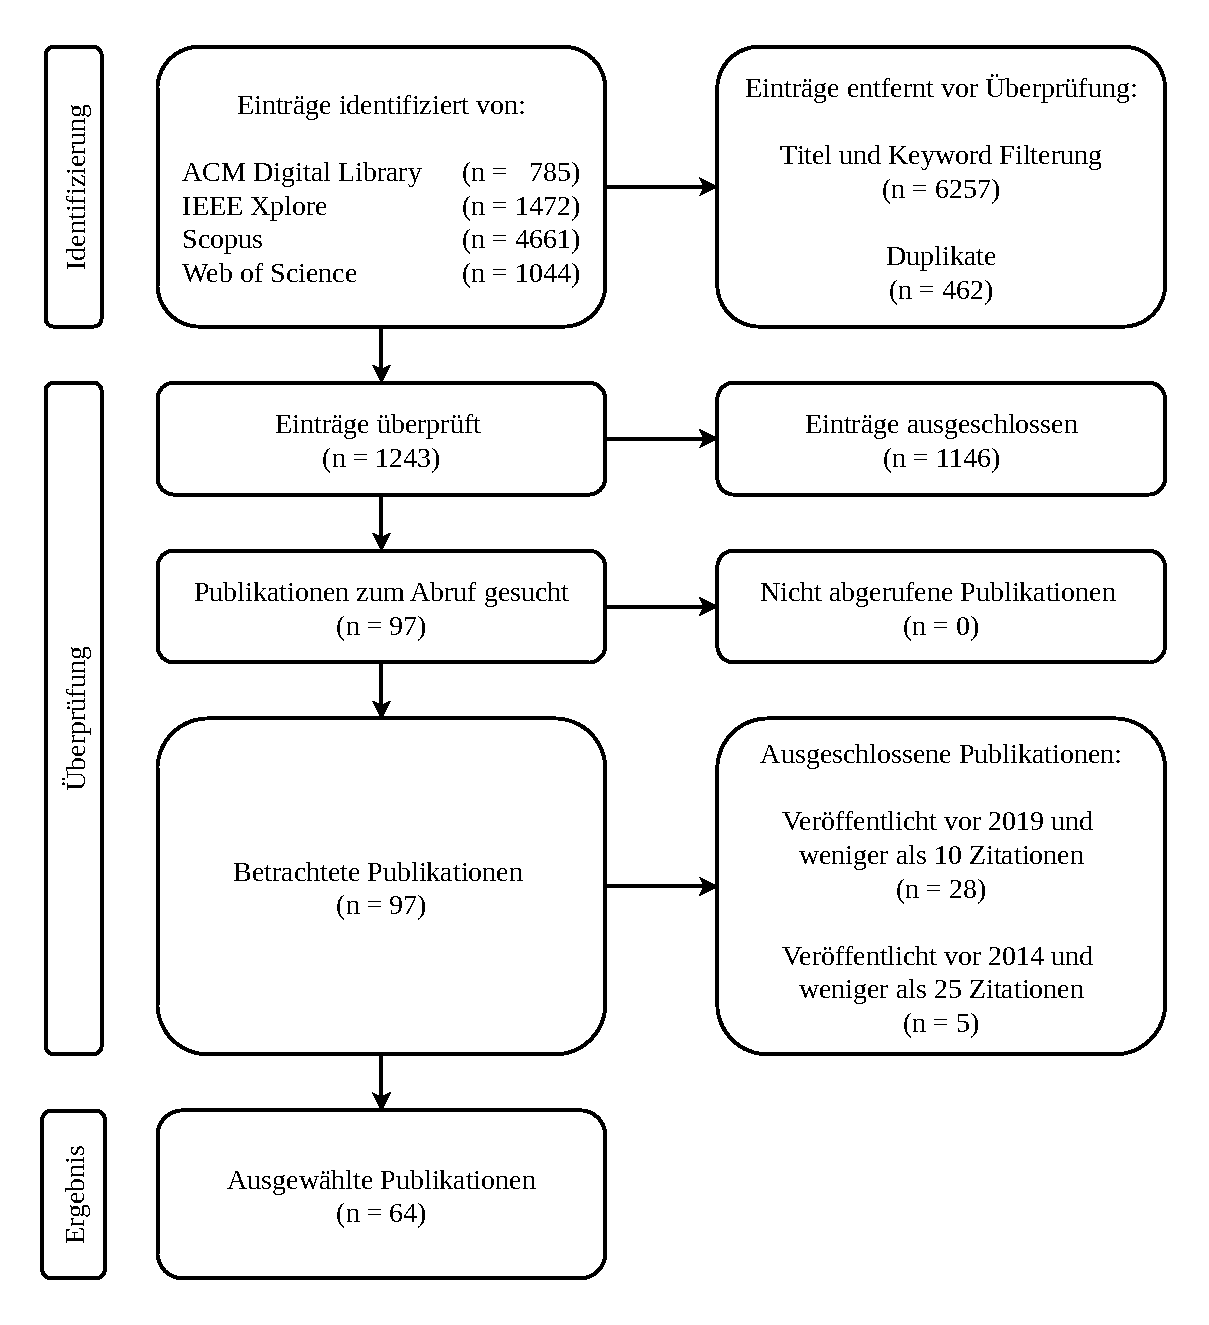
\includegraphics[width=\textwidth]{diagrams/PRISMA.pdf}
    \caption{PRISMA Diagramm}
    \label{prisma-diagram}
\end{figure}

Die Publikationen beschreiben eine Vielzahl an verschiedenen webbasierten integrierten Entwicklungsumgebungen. Dabei kann eine Unterteilung in die folgenden zwei Kategorien erfolgen:

\begin{itemize}
    \item \textbf{Client-Server-basierte Lösungen} \\
          Systeme dieser Art zeichnen sich dadurch aus, dass sie eine Client-Server-Archi-tektur verwenden. Hierbei werden Features, die nicht innerhalb eines Browsers ausgeführt werden können (z.B. Kompilierung) über einen entsprechenden Server bereitgestellt.
    \item \textbf{Browser-basierte Lösungen} \\
          Systeme dieser Art zeichnen sich dadurch aus, dass alle Features im Browser des Nutzers ausgeführt werden können, ohne die Hilfe eines separaten Servers.
\end{itemize}

Deursen et al. (2010) \cite{van_deursen_adinda_2010} beschreiben eine online IDE names Adinda. Die grundlegende Idee von Adinda ist die Zerlegung der Funktionalität einer IDE in einen leichtgewichtigen Client sowie mehrere zusammenarbeitende (Web-)Services. Diese Services sollen dann bestimmte Aufgaben erfüllen, wie z.B. Kompilierung, Testen, kollaboratives Editieren und Datenerhebung. Es werden weiterhin verschiedenste Forschungsfragen aufgestellt, die für das vorgestellte System von Interesse sind. Die prototypische Implementierung von Adinda basiert auf WWWorkspace \cite{ryan_web_2007} und nutzt serverseitig Eclipse \cite{noauthor_eclipse_nodate}. Der Prototyp unterstützt das Erstellen von Nutzer-Workspaces, Java Projekten, Paketen und Klassendateien sowie Syntax Highlighting, Kompilierung und Code-Vervollständigung. \todo{Adinda} \\

Wu et al. (2011) \cite{wu_ceclipse_2011} stellen die online IDE Cloud Eclipse (CEclipse) vor. Die Ziele von CEclipse sind:
\begin{enumerate}
    \item die Bereitstellung von Eclipse \cite{noauthor_eclipse_nodate} Funktionen wie z.B. Code-Vervollständigung
    \item die Behandlung von den online IDE spezifischen Sicherheitsproblemen \quoted{\textit{Wrong file operations}}, \quoted{\textit{Banned operation calling}} und \quoted{\textit{Excessive resource consumption}}
    \item die Ausnutzung von Cloud Computing Möglichkeiten um Entwickler besser zu unterstützen.
\end{enumerate} 
Für $1.$ wurde ein entsprechendes Protokoll entwickelt, was es ermöglicht die gewünschten Funktionen von Eclipse aufzurufen und das Ergebnis im Browser darzustellen. Um die in $2.$ genannten Probleme Handhaben zu können wird ein \textit{Program Behavior Analysis Service} beschrieben. Durch die Einschränkung des Dateisystems auf einen speziellen Ordner kann das Problem \quoted{Wrong file operations} gelöst werden. Das Verbieten bzw. Erlauben von Methoden über eine Blacklist bzw. eine Whitelist kann zur Lösung des Problems \quoted{Banned operation calling} angewendet werden. Durch eine Zeitbegrenzung von laufenden Prozessen kann schließlich auch das Problem \quoted{Excessive resource consumption} behoben werden. Für $3.$ werden über den \textit{Program Behavior Mining Service} Daten über die Nutzung der IDE gesammelt werden. Diese Daten können dann z.B. dazu genutzt werden dem Entwickler häufig verwendete Befehle mit höherer Priorität vorzuschlagen. \todo{CEclipse} \\

Goldman et al. (2011) \cite{goldman_real-time_2011} beschreiben Collabode, eine kollaborative online IDE für Java. Collabode ermöglicht es mehreren Nutzern gleichzeitig Änderungen an Dateien vorzunehmen. Die Änderungen werden in Echtzeit zwischen den Nutzern synchronisiert. Dabei wird ein spezieller Algorithmus verwendet. Dieser Algorithmus sorgt dafür, dass nur Änderungen eingepflegt werden, die keinen syntaktischen Fehler beinhalten oder erzeugen. Dadurch wird sichergestellt, das Nutzer nur ihre eigenen Fehler sehen und das Programm unabhängig von den ggf. vorhandenen Fehlern ihrer Teammitglieder kompilieren können. Collabode nutzt EtherPad \cite{noauthor_etherpad_nodate} als Editor im Frontend und Eclipse \cite{noauthor_eclipse_nodate} für die Bereitstellung von Kompilierung, Syntax Highlighting, etc. im Backend. \todo{Collabode} \\

Lautamäki et al. (2012) \cite{lautamaki_cored_2012} stellen Collaborative Real-time Editor (CoRED) vor, einen online Code Editor für Java Programme. CoRED nutzt den ACE Editor \cite{noauthor_ace_nodate} im Fronted sowie das Java Development Kit (JDK) \todoaddref[]{JDK} zur Kompilierung im Backend. Fehlermeldungen während des Kompiliervorgangs werden an den Client zurückgesendet und dann im Frontend visualisiert. Zur Bereitstellung von Echtzeit Kollaboration wird der Algorithmus \textit{Differential Synchronization with shadows} \cite{fraser_differential_2009} von Neil Fraser eingesetzt. Ein weiteres Feature von CoRED ist das Sperren von Code Bereichen für andere Nutzer sowie die Möglichkeit Kommentare im Code zu hinterlassen. Auf diese Kommentare können dann andere Nutzer antworten, wodurch eine weitere Interaktionsmöglichkeit besteht. Weiterhin bietet CoRED auch Code-Vervollständigung an. \todo{CoRED} \\

Ball et al. (2015) \cite{ball_beyond_2015} beschreiben TouchDevelop. TouchDevelop ist eine online IDE bzw. eine cloudbasierte IDE (CIDE). Das Hauptfeature von TouchDevelop ist die Speicherung aller Programmänderungen, Versionen, Laufzeitinformationen, Bugs sowie Kommentare, Fragen und Feedback von Nutzern in einer zentralen Datenbank. Diese Daten können über entsprechende APIs abgefragt werden. Die Nutzeroberfläche von TouchDevelop unterscheidet sich stark von anderen textbasierten Editoren. So bekommt der Nutzer eine Auswahl an kontextabhängigen Optionen, z.B. if-Anweisungen, for-Schleifen oder verfügbare Variablen. Alle IDE Funktionen sind offline verfügbar, da sie komplett auf der Clientseite implementiert sind. Weiterhin nutzt TouchDevelop eine eigene Programmiersprache. Diese folgt dem imperativen Programmierparadigma, besitzt ein starkes Typsystem sowie eine Vielzahl an plattformübergreifenden APIs. \dots \todo{TouchDevelop} \\

Tran et al. (2013) \cite{tran_interactive_2013} \dots \\
Nguyen et al. (2014) \cite{nguyen_learning_2014} \dots \\
Nguyen et al. (2016) \cite{nguyen_enhancing_2016} \dots \todo{IDEOL/EduCo} \\

Warner und Guo (2017) \cite{warner_codepilot_2017} \dots \todo{CodePilot} \\

Über mehrere Publikationen wird die Entwicklung der Reflex IDE (RIDE) beschrieben.  Zunächst wird von Bastrykina et al. (2021) \cite{bastrykina_developing_2021} ein entsprechender Kernel mit dem Xtext Framework \cite{noauthor_xtext_nodate} entwickelt, welcher in der Eclipse IDE verwendet werden kann, um diese \todo{}. Darauf aufbauend wird von Gornev und Liakh (2021) \cite{gornev_ride_2021} die Konzipierung und Implementierung einer auf Theia basierten Web-Variante von RIDE vorgestellt. Gornev et al. (2022) \cite{gornev_towards_2022} beschreiben ein System, welches Docker verwendet um die Web-Version von RIDE für mehrere simultane Nutzer bereitstellen zu können. Gornev und Bondarchuk (2023) \cite{gornev_towards_2023} entwickeln ein Framework, welches es erlaubt Echtzeit-Kollaboration in Single-User Anwendungen zu ermöglichen. Kuznetsov und Zyubin (2024) \cite{kuznetsov_development_2024} beschreiben die Entwicklung eines Projektmanagement-Systems für RIDE. \todo{RIDE} \\

Jefferson et al. (2024) \cite{jefferson_pyodideu_2024} beschreiben eine IDE, die es Nutzern ermöglicht Python Code im Browser zu schreiben und auszuführen. Dabei wird das Programm des Nutzers lokal in dessem Browser durchgeführt. Dies wird durch den Einsatz von PyodideU erreicht, einer erweiterten Version der WebAssembly-basierten Python Distribution Pyodide \cite{noauthor_pyodide_nodate}. Zusätzlich wird den Nutzern auch eine Grafikbibliothek angeboten samt eines Debuggers, der es ermöglicht Zeile für Zeile und auch rückwärts durch das Programm zu gehen und die entsprechenden Änderungen an der Grafik zu sehen. Weiterhin wird durch PyodideU auch die synchrone Eingabe von Daten unterstützt, während Python im Main-Thread des Browsers läuft. Zudem wird auch ein Dateisystem bereitgestellt. Insgesamt wurde die IDE sowohl von Studenten als auch von Lehrenden als hilfreich wahrgenommen. \todo{PyodideU} \\

Malan (2024) \cite{malan_containerizing_2024} beschreibt die verschiedenen Ansätze zur Bereitstellung einer integrierten Entwicklungsumgebung für die Teilnehmer des Einführungskurses in die Programmierung (CS50) an der Harvard University. Zunächst wurde seit 2007 ein On-Campus Cluster für die Studenten angeboten. Studenten konnten über SSH mit diesem verbinden und dort ihre Programme ausführen. Dieser Cluster wurde 2008 mithilfe von Amazon Web Services (AWS) \cite{noauthor_amazon_nodate} in die Cloud überführt. Diese cloud-basierte Lösung wurde 2011 durch Client-seitige virtuelle Maschinen ersetzt. In 2015 wurde eine auf Docker basierende Lösung erarbeitet, die zunächst Cloud9 IDE \cite{noauthor_cloud_nodate} als Frontend nutzte. In 2021 wurde schlielich eine auf Github Codespaces aufbauende Lösung eingeführt, die VSCode als Code Editor verwendet. \todo{CS50} \\

\todo{Vorteile von online IDEs}

\todo{Nachteile von online IDEs}

\todo{Anforderungen an online IDEs}

\section{Weitere online IDEs} \label{weitere-online-ides}

% opt: zusätzliche Anhänge
\begin{appendix}
    % \input{content/anhang1}
\end{appendix}

% --- Abbildungs-, Tabellen-, Algorithmen- und Literaturverzeichnis ------------
\backmatter
% Abbildungsverzeichnis
\listoffigures
% Tabellenverzeichnis
\listoftables
% Algorithmenverzeichnis
\listofalgorithms
% Literaturverzeichnis
\cleardoublepage	% Literaturverzeichnis immer auf ungerader Seite
\phantomsection		% Anker für Sprungmarke im Inhaltsverzeichnis korrigieren
\addcontentsline{toc}{chapter}{\bibname}
\bibliography{NIKR_bibliography}
\end{document}
